% !TeX TS-program = xelatex

\documentclass[12pt,aspectratio=169]{beamer}
\usepackage{graphicx}
\usepackage{xcolor}
\usepackage{fontspec}
\usepackage{tikz}
\usepackage{caption}
\usepackage{subfig}

\setsansfont{EB Garamond}
\definecolor{primarycolor}{RGB}{0, 96, 157}

\setbeamertemplate{itemize item}{\color{primarycolor}$\bullet$}
\setbeamertemplate{itemize subitem}{\color{primarycolor}$\blacktriangleright$}

\usepackage{setspace}
\setstretch{1.3}

\captionsetup{
	format=plain,
	justification=raggedright,
	singlelinecheck=false,
	font={normalsize,color=primarycolor},
	labelfont={color=primarycolor},
	labelsep=space,
	skip=0pt
}

\title{Boletim de Conjuntura Econômica do Tocantins 2020}
\subtitle{v 9, nº1}
\author{PET Economia}
\institute{Universidade Federal do Tocantins}
\date{26/03/2021}

\begin{document}
\setbeamercolor{title}{fg=white}
\setbeamercolor{background canvas}{bg=primarycolor}
\setbeamercolor{normal text}{fg=white}
\usebeamercolor[fg]{normal text}
\begin{frame}
    \begin{tikzpicture}[overlay]
        \node[anchor=center] at (3,-3){
\includegraphics[width=7cm]{bg.pdf}};
    \end{tikzpicture}
    \titlepage
\end{frame}

\setbeamercolor{background canvas}{bg=white}
\setbeamercolor{normal text}{fg=black}
\setbeamercolor{title}{fg=red}
\usebeamercolor[fg]{normal text}
\setbeamercolor{frametitle}{fg=primarycolor,bg=white}

\begin{frame}  
\frametitle{Introdução}
\begin{itemize}
\item O Boletim é uma publicação semestral
\item Apresentar a evolução das principais variáveis macroeconômicas do estado durante o semestre em análise
\item Metodologia
\item Todo o processo de construção está disponível no GitHub \url{https://github.com/peteconomia/boletim}
\item Divulgado pelo CORECON--TO \url{https://corecon-to.org.br/boletins-de-conjuntura/}
\end{itemize}
\end{frame}

\begin{frame}
    \frametitle{Panorama Econômico}
    \begin{itemize}
        \item Expectativas captadas pelo Boletim Focus do Banco Central
    \end{itemize}

	\begin{figure}%
		\centering
		\subfloat[\centering Expectativas de Crescimento do PIB para 2020]{{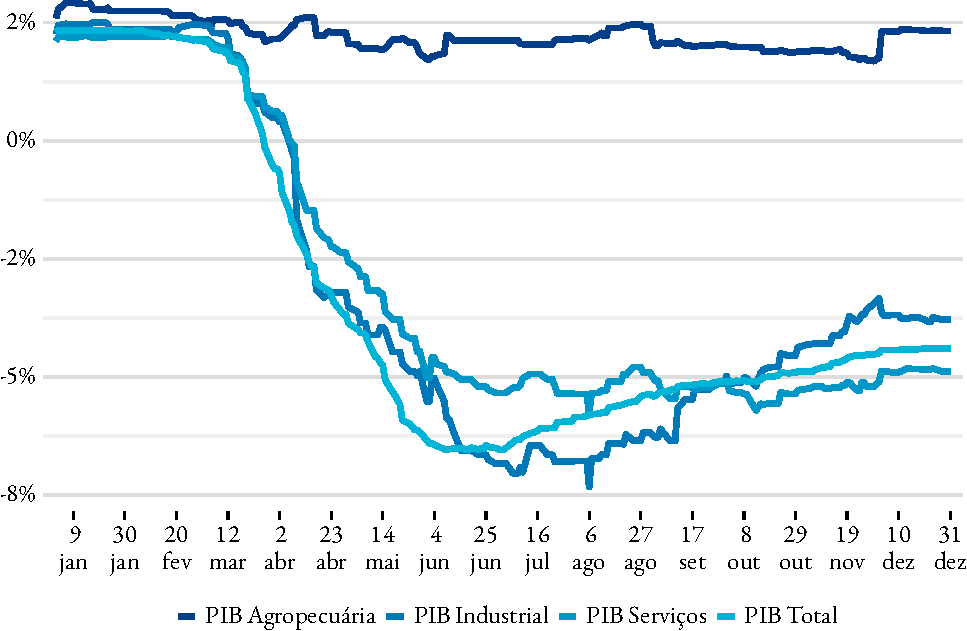
\includegraphics[width=.45\textwidth]{figs/PIB.pdf} }}%
		%\qquad
		%\subfloat[\centering Pesquisa Mensal do Comércio]{{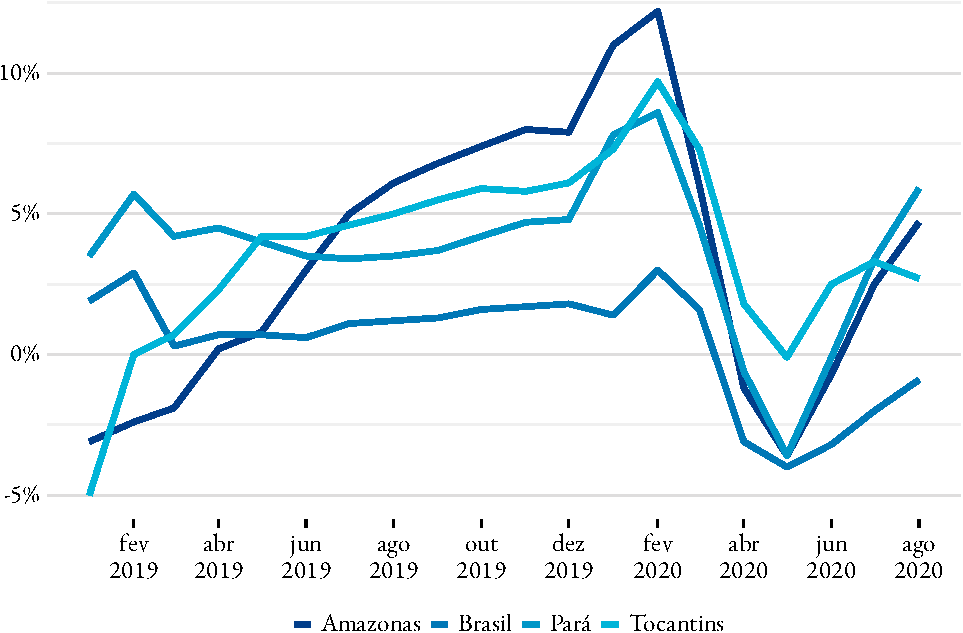
\includegraphics[width=.45\textwidth]{figs/PMC.pdf} }}%
	\end{figure}



\end{frame}
\begin{frame}
	\frametitle{Panorama Econômico}
	\begin{itemize}
		\item Impacto da COVID-19 na atividade econômica
		\item O resultado final em 2020 foi de uma queda de 4,1\%

	\end{itemize}
	
	\begin{figure}%
		\centering
		\subfloat[\centering Resultado Trimestral do PIB pelo Lado da Demanda]{{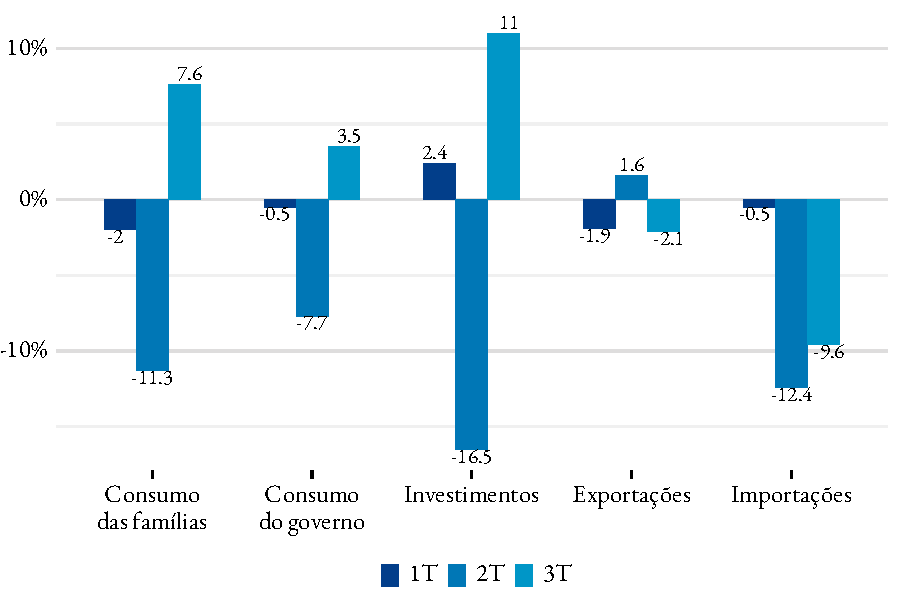
\includegraphics[width=.45\textwidth]{figs/pib_demanda.pdf} }}%
		\qquad
		\subfloat[\centering Resultado Trimestral do PIB pelo Lado da Oferta]{{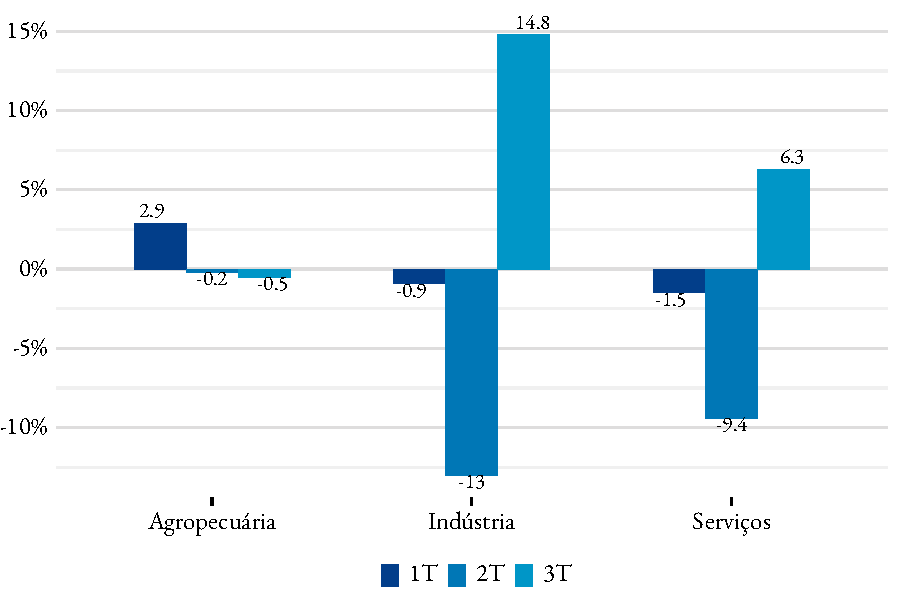
\includegraphics[width=.45\textwidth]{figs/pib_oferta.pdf} }}%
	\end{figure}
\end{frame}
\begin{frame}
	\frametitle{Panorama Econômico}
	\begin{itemize}
		\item Atividade econômica no Tocantins
		\item Crescimento, comércio e serviços
	\end{itemize}
	
	\begin{figure}%
		\centering
		%\subfloat[\centering Expectativas de Crescimento do PIB para 2020]{{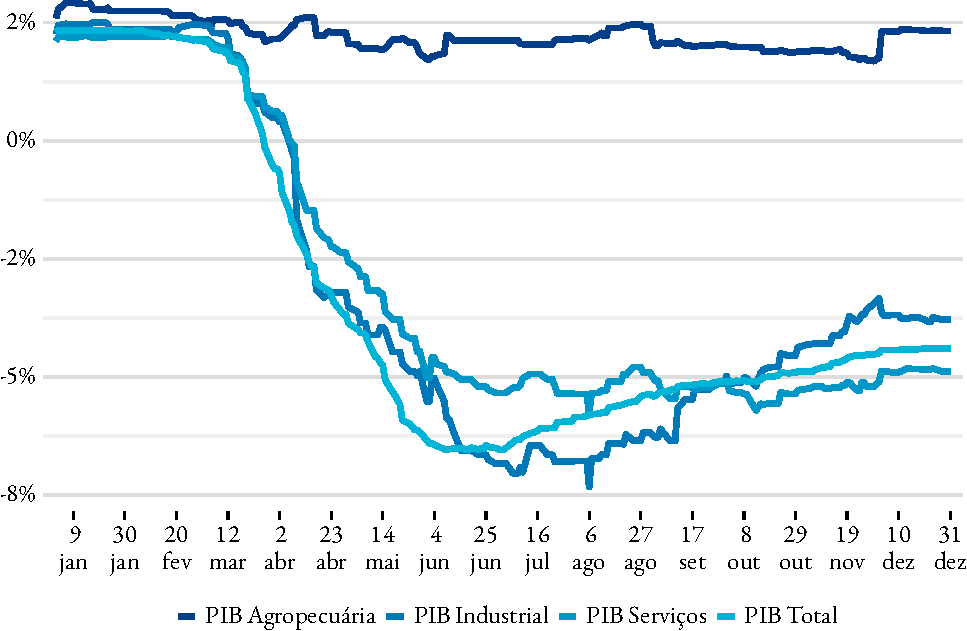
\includegraphics[width=.45\textwidth]{figs/PIB.pdf} }}%
		%\qquad
		\subfloat[\centering Pesquisa Mensal do Comércio]{{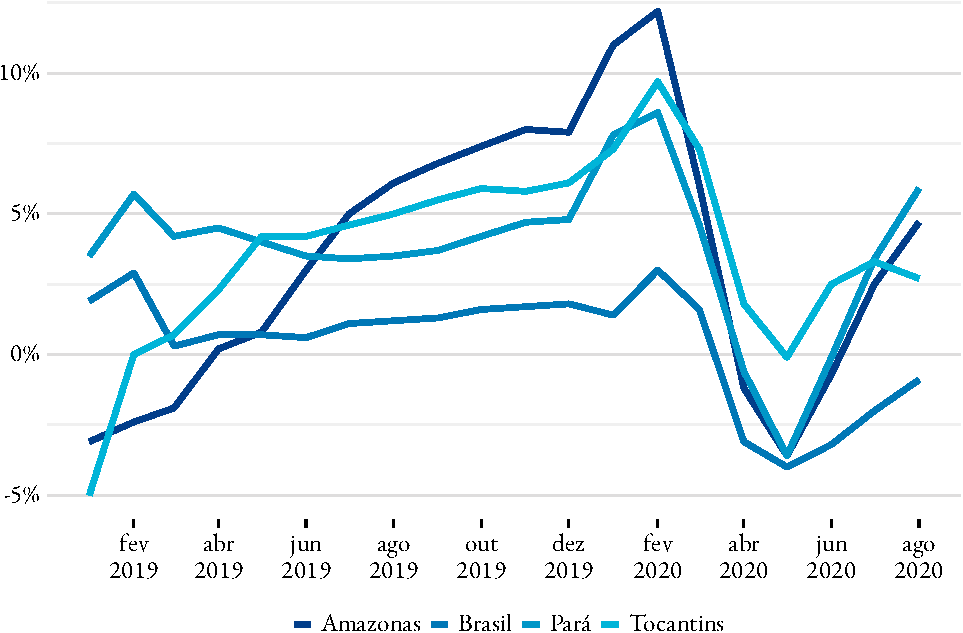
\includegraphics[width=.45\textwidth]{figs/PMC.pdf} }}%
	\end{figure}	
\end{frame}

\begin{frame}
	\frametitle{Contas Públicas Estadual}
	\begin{itemize}
		\item Situação fiscal do estado, principais indicadores
		\item Resultado primário de R\$ 1,08 bilhões, valor 73\% que no mesmo período de 2019
		\item Despesa total com pessoal
		\item Dívida consolidada
		\item Limites de endividamento
		\item Capacidade de Pagamento
	\end{itemize}
\end{frame}

\begin{frame}
    \frametitle{Contas Públicas Estadual}
    \begin{figure}%
        \centering
        \subfloat[\centering Despesa total com pessoal em relação à RCL]{{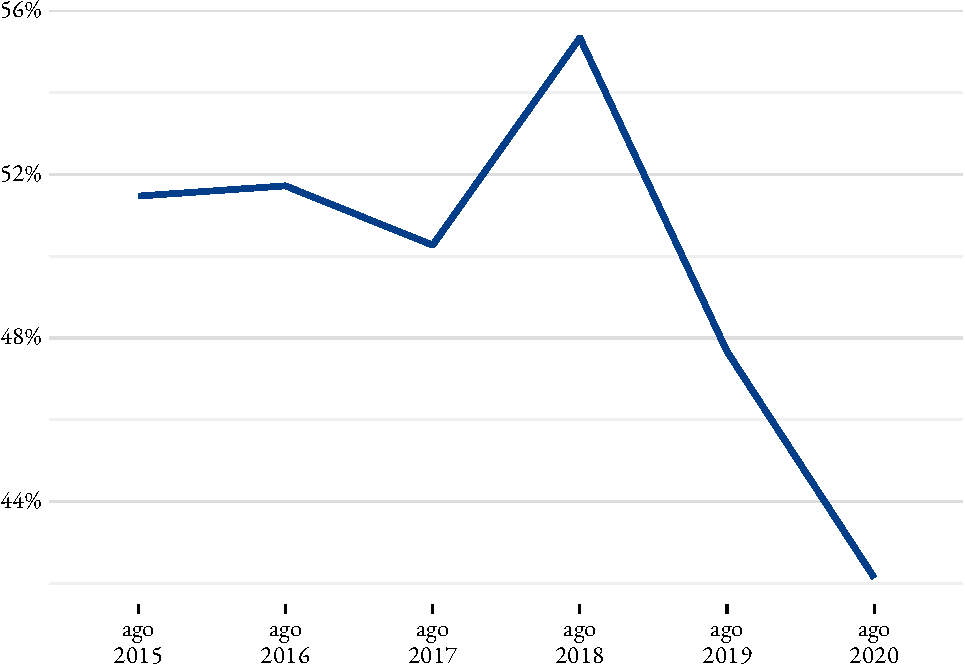
\includegraphics[width=.45\textwidth]{figs/desp_pessoal_rcl-1.pdf} }}%
        \qquad
        \subfloat[\centering Dívida Consolidada Líquida em relação à RCL]{{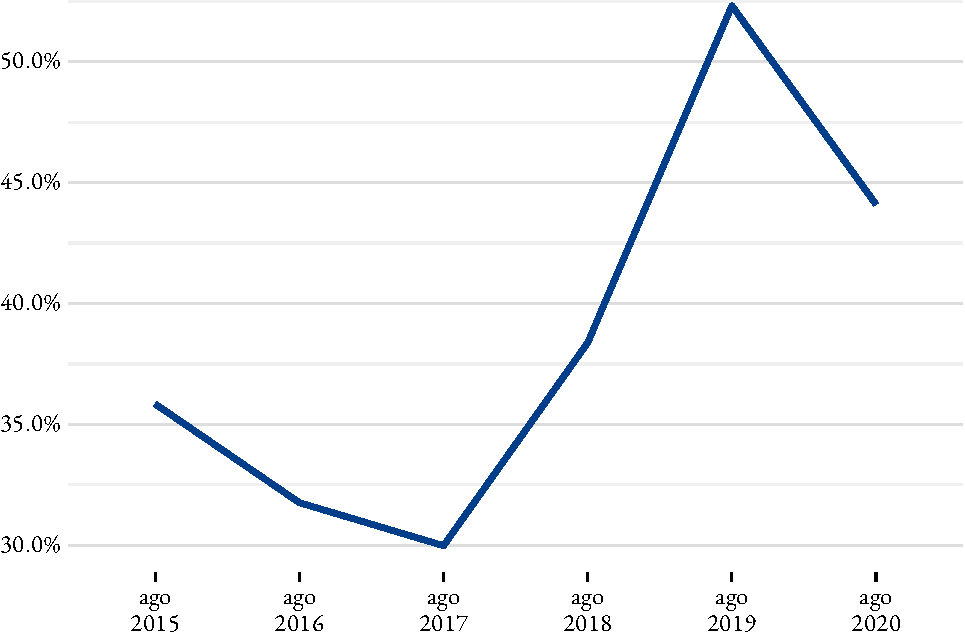
\includegraphics[width=.45\textwidth]{figs/divida_rcl-1.pdf} }}%
    \end{figure}
\end{frame}

\begin{frame}
	\frametitle{Indicadores Sociais}
	\begin{itemize}
		\item Taxa de pobreza caiu no Tocantins, apesar da taxa brasileira ter andado de lado 
		\item Extrema pobreza vem crescendo
		
	\end{itemize}
	
	\begin{figure}%
		\centering
		\subfloat[\centering Taxa de Pobreza - Linha de US\$5,50 PPC]{{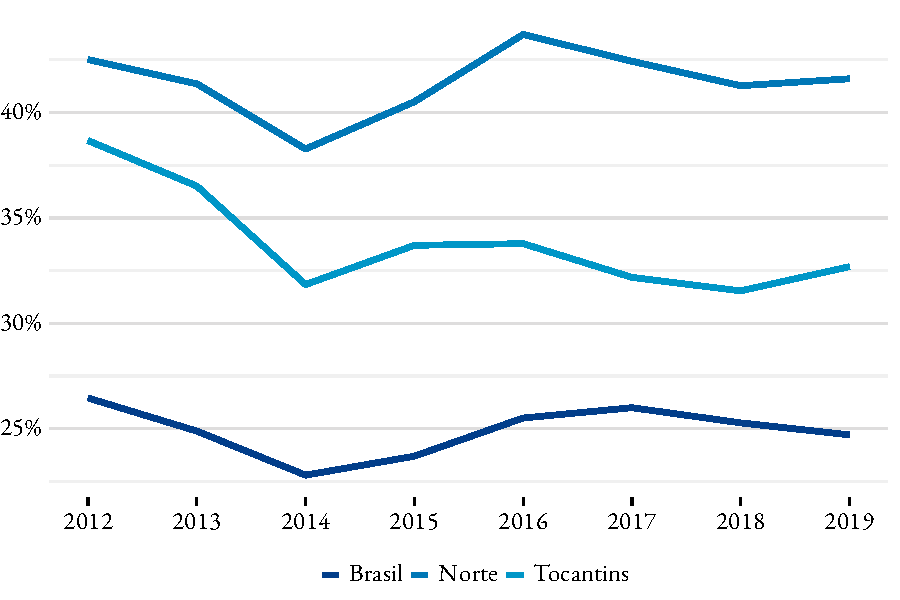
\includegraphics[width=.45\textwidth]{figs/taxa_pobreza.pdf} }}%
		\qquad
		\subfloat[\centering Taxa de Extrema Pobreza - Linha de US\$1,90 PPC]{{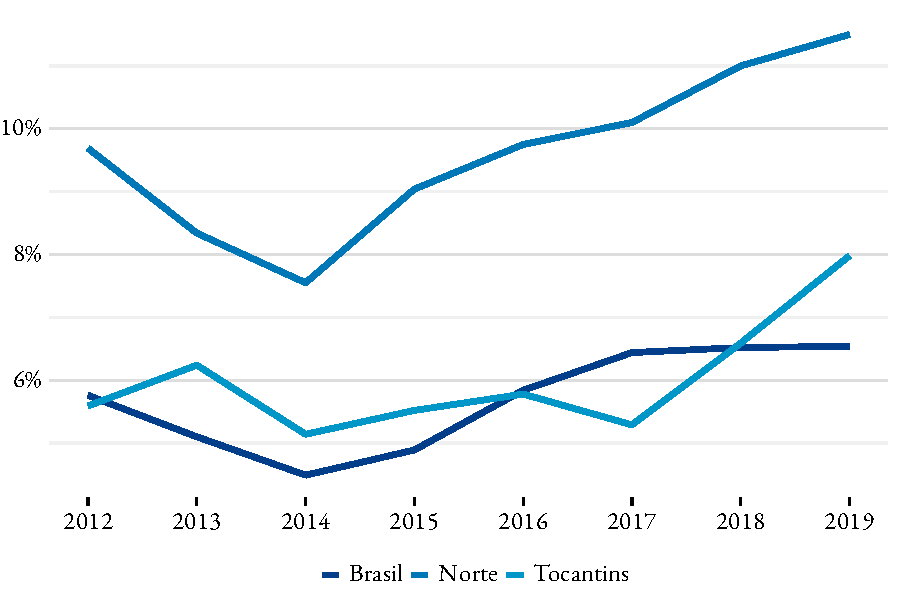
\includegraphics[width=.45\textwidth]{figs/taxa_expobreza.pdf} }}%
	\end{figure}
\end{frame}

\begin{frame}
	\frametitle{Indicadores Sociais}
	\begin{itemize}
		\item Desigualdade tem aumentado no Tocantins
	\end{itemize}
	
	\begin{figure}%
		\centering
		\subfloat[\centering Índice de Gini]{{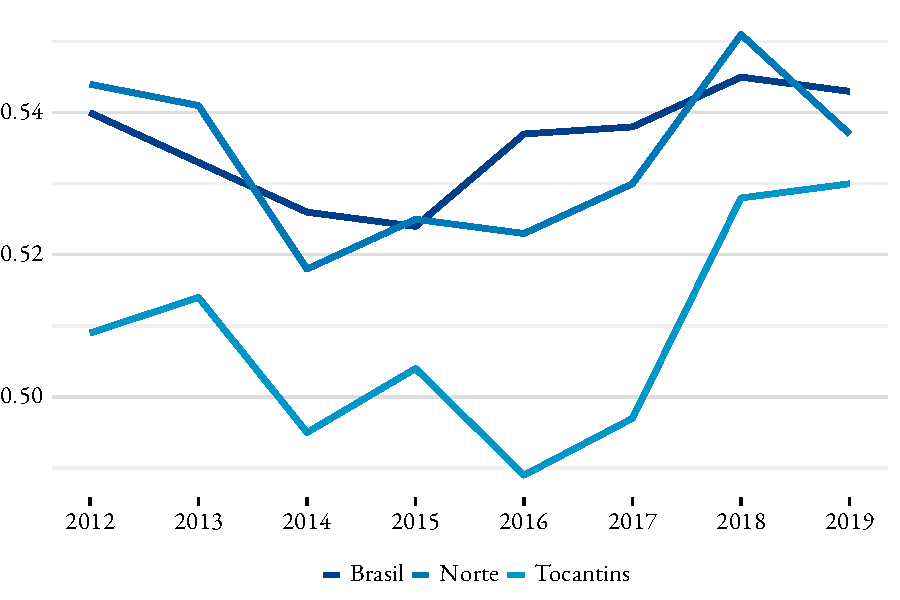
\includegraphics[width=.45\textwidth]{figs/gini.pdf} }}%
	\end{figure}	
\end{frame}

\begin{frame}
	\frametitle{Mercado de Trabalho}
	
	\begin{itemize}
		\item Desempenho do mercado de trabalho formal a partir do CAGED e PNAD-C
		\item Saldo de empregos
	\end{itemize}

\begin{figure}%
	\centering
	\subfloat[\centering Saldo de empregos ao longo de 2020]{{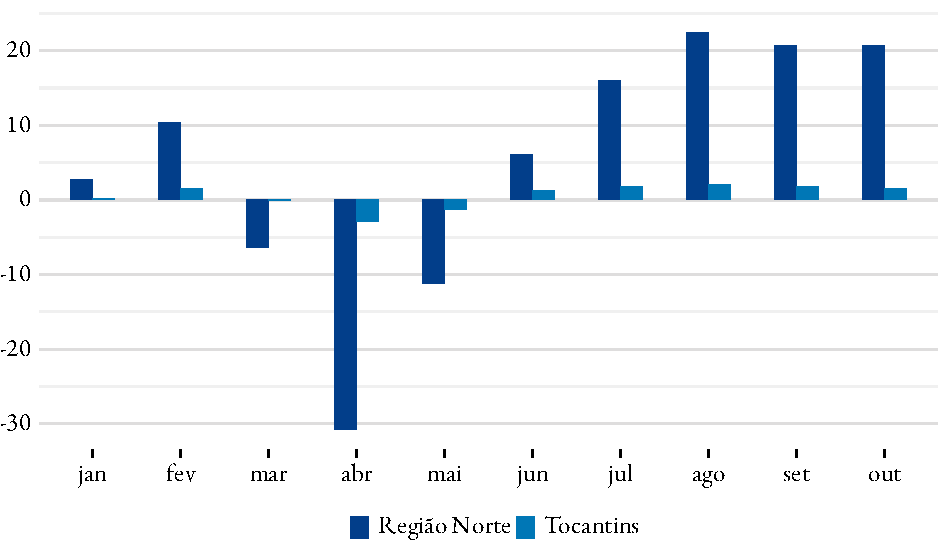
\includegraphics[width=.45\textwidth]{figs/Setores.pdf}}}%
	\qquad
	\subfloat[\centering Saldo por setores]{{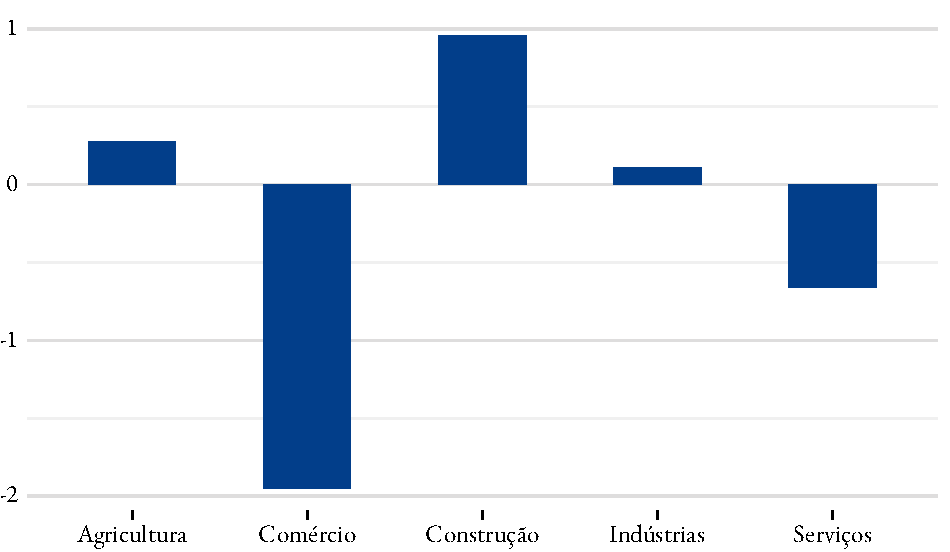
\includegraphics[width=.45\textwidth]{figs/saldo_por_setores.pdf} }}%
	
\end{figure}
\end{frame}

\begin{frame}
	\frametitle{Mercado de Trabalho}
\begin{itemize}
	\item Perfil dos admitidos e demitidos, além da questão do gênero e etnia
	\item A desigualdade no mercado de trabalho formal
	\item Taxa de desemprego, população ocupada e rendimento médio real
\end{itemize}

\begin{figure}%
	\centering
	\subfloat[\centering Taxa de desemprego]{{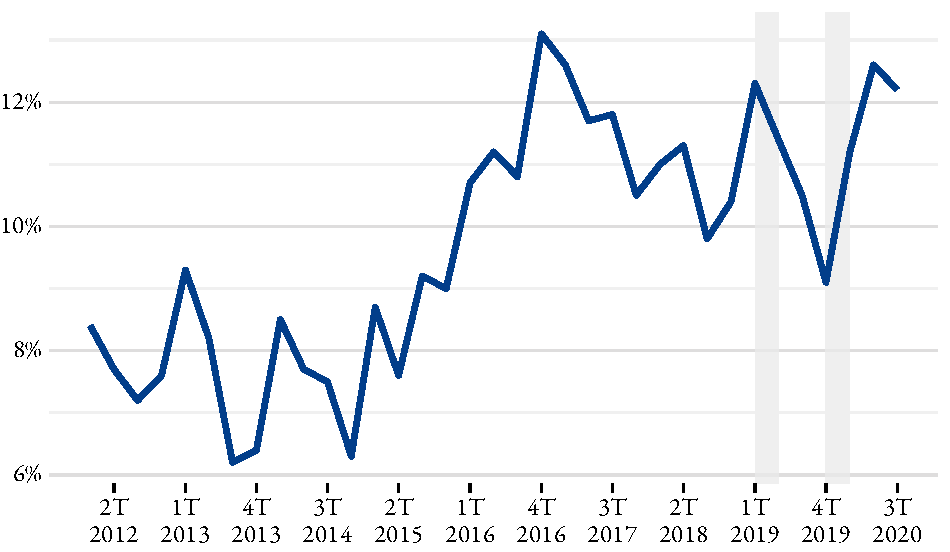
\includegraphics[width=.45\textwidth]{figs/taxa_desemprego.pdf}}}%
	\qquad
	\subfloat[\centering População ocupada]{{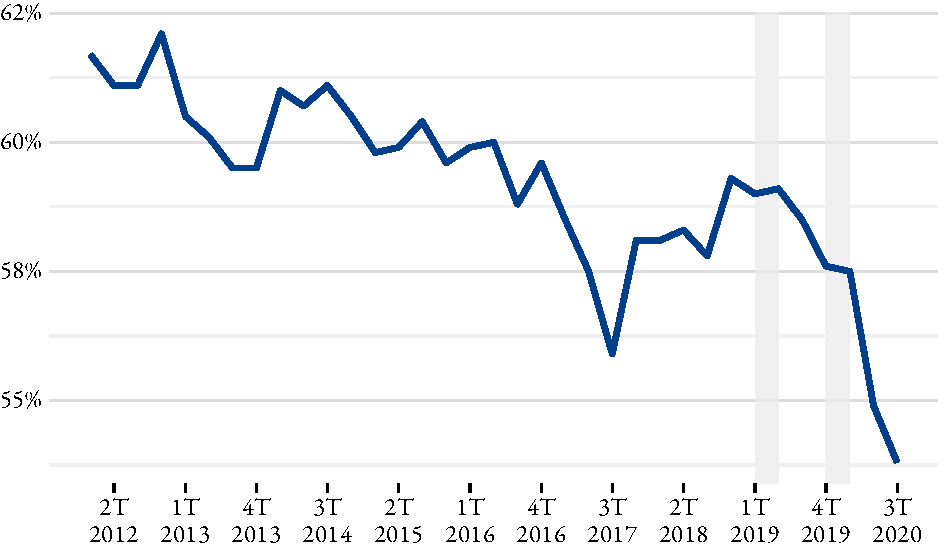
\includegraphics[width=.45\textwidth]{figs/pop_ocupada.pdf} }}%
	
\end{figure}


\end{frame}

\begin{frame}
	\frametitle{Mercado de Trabalho}
	\begin{itemize}
		\item Rendimento médio real
		\item Exposições do mercado de trabalho
	\end{itemize}
	
	\begin{figure}%
		\centering
		\subfloat[\centering Taxa de desemprego]{{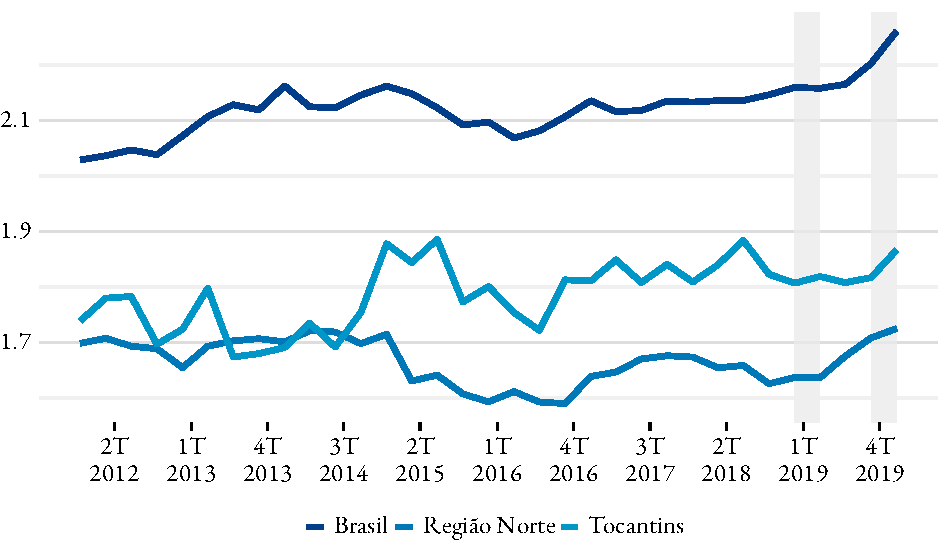
\includegraphics[width=.45\textwidth]{figs/rendimentos.pdf}}}%
		\qquad
		\subfloat[\centering Perfil dos Admitidos e demitidos ocupada]{{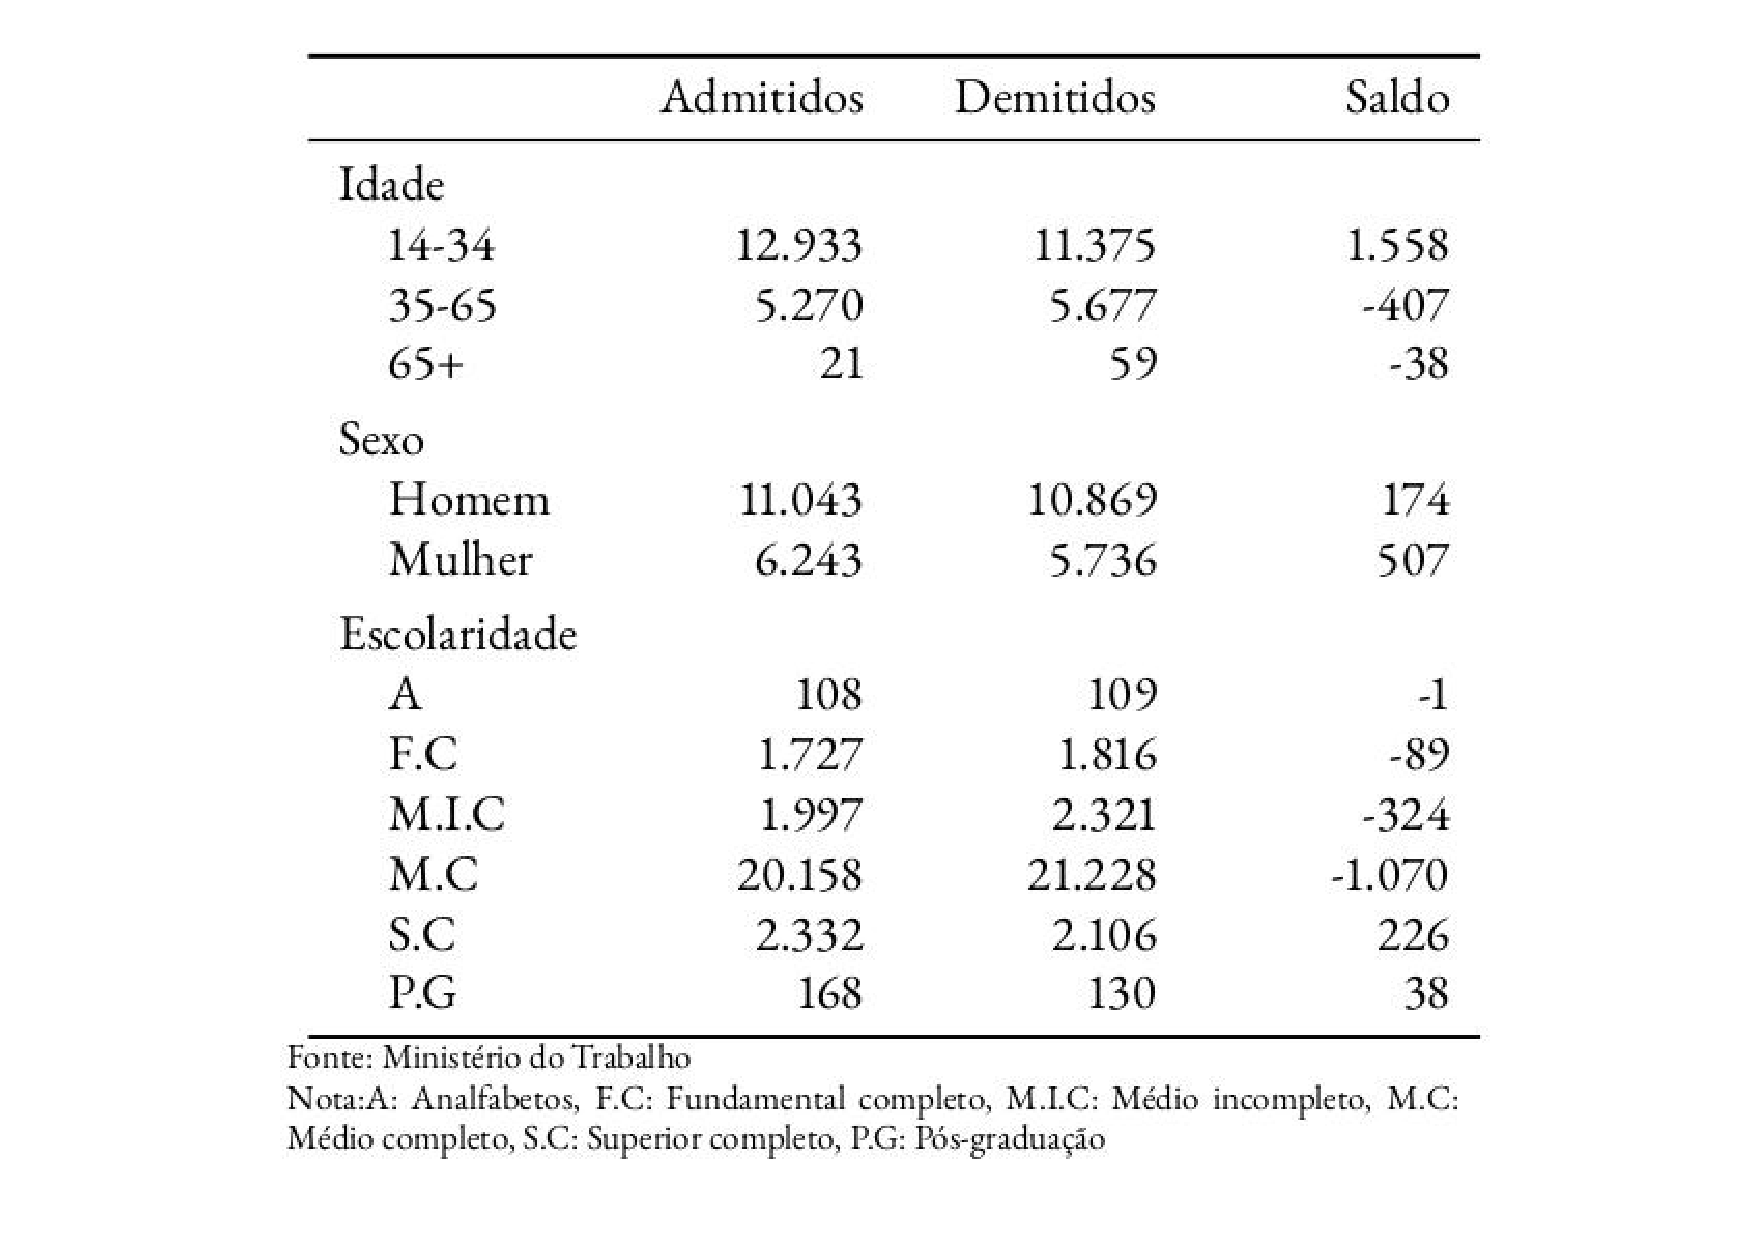
\includegraphics[width=.45\textwidth]{figs/tabelaEmp.pdf} }}%
		
	\end{figure}
	
	
\end{frame}



\begin{frame}
	\frametitle{Comércio Exterior}
	\begin{itemize}
		\item Série histórica dos valores gerais
	\end{itemize}

\begin{figure}%
	\centering
	\subfloat[\centering Valores Gerais]{{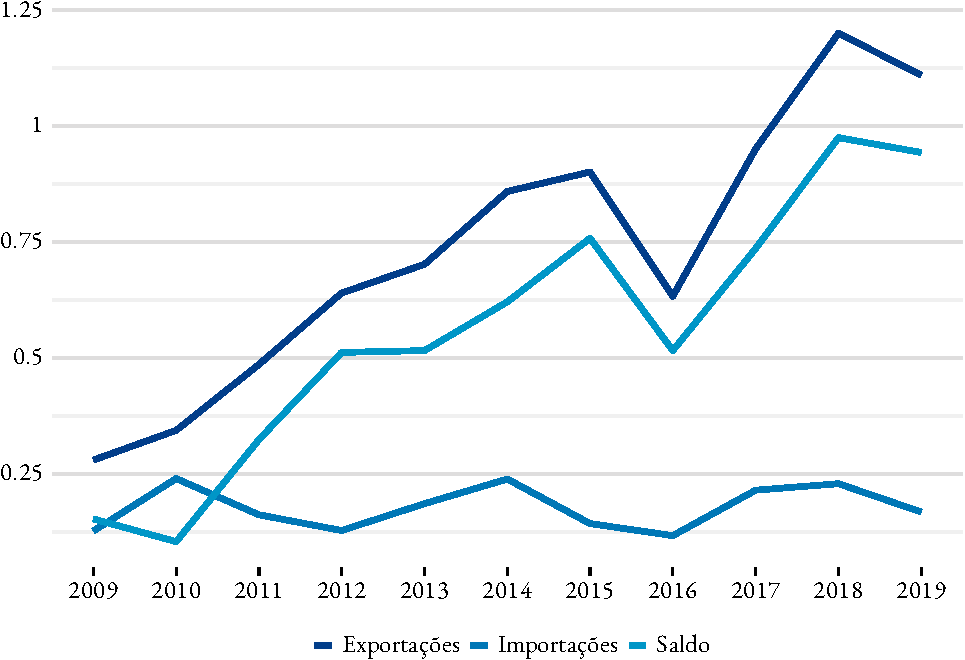
\includegraphics[width=.45\textwidth]{figs/total bc.pdf}}}%
	
\end{figure}
\end{frame}

\begin{frame}
	\frametitle{Comércio Exterior}
	\begin{itemize}
		\item Exportação e Importação
	\end{itemize}
	
	\begin{figure}%
		\centering
		\subfloat[\centering Produtos exportados]{{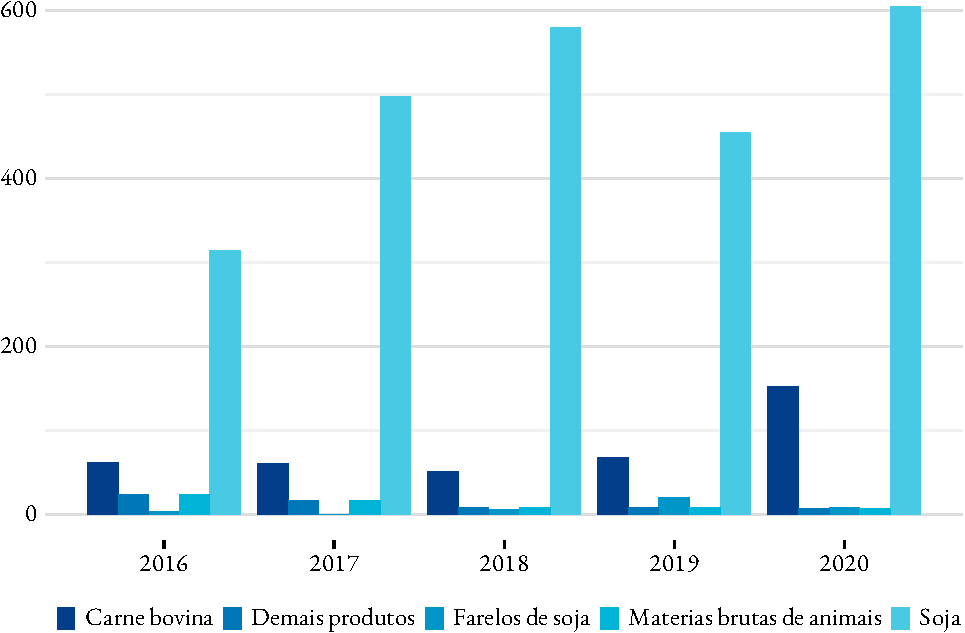
\includegraphics[width=.45\textwidth]{figs/export1.pdf}}}%
		\qquad
\subfloat[\centering Produtos importados]{{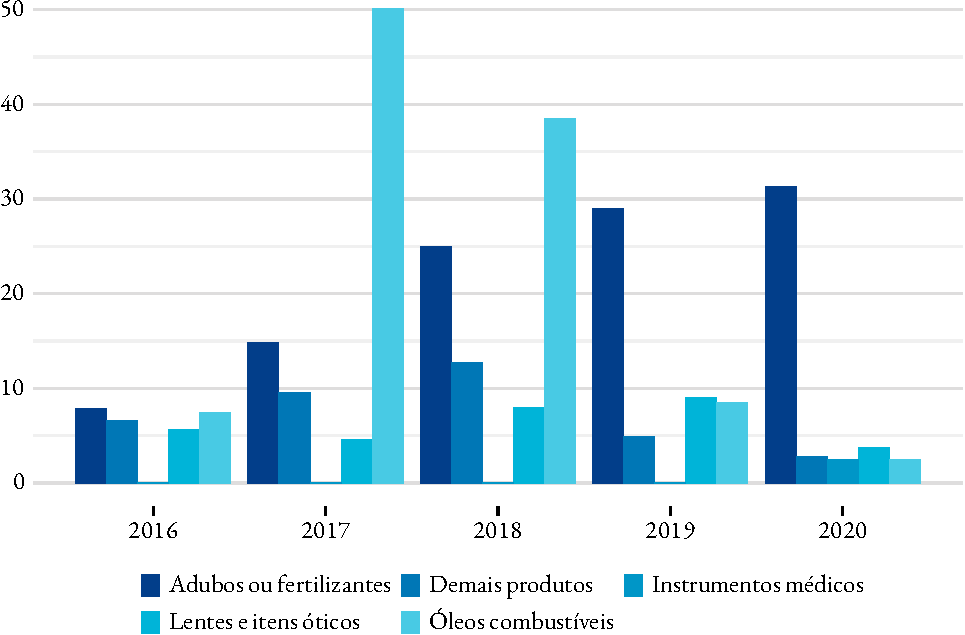
\includegraphics[width=.45\textwidth]{figs/import1.pdf} }}%
	\end{figure}
\end{frame}

\begin{frame}
	\frametitle{Comércio Exterior}
	\begin{itemize}
		\item Países Parceiros
	\end{itemize}
	
	\begin{figure}%
		\centering
		\subfloat[\centering Destino]{{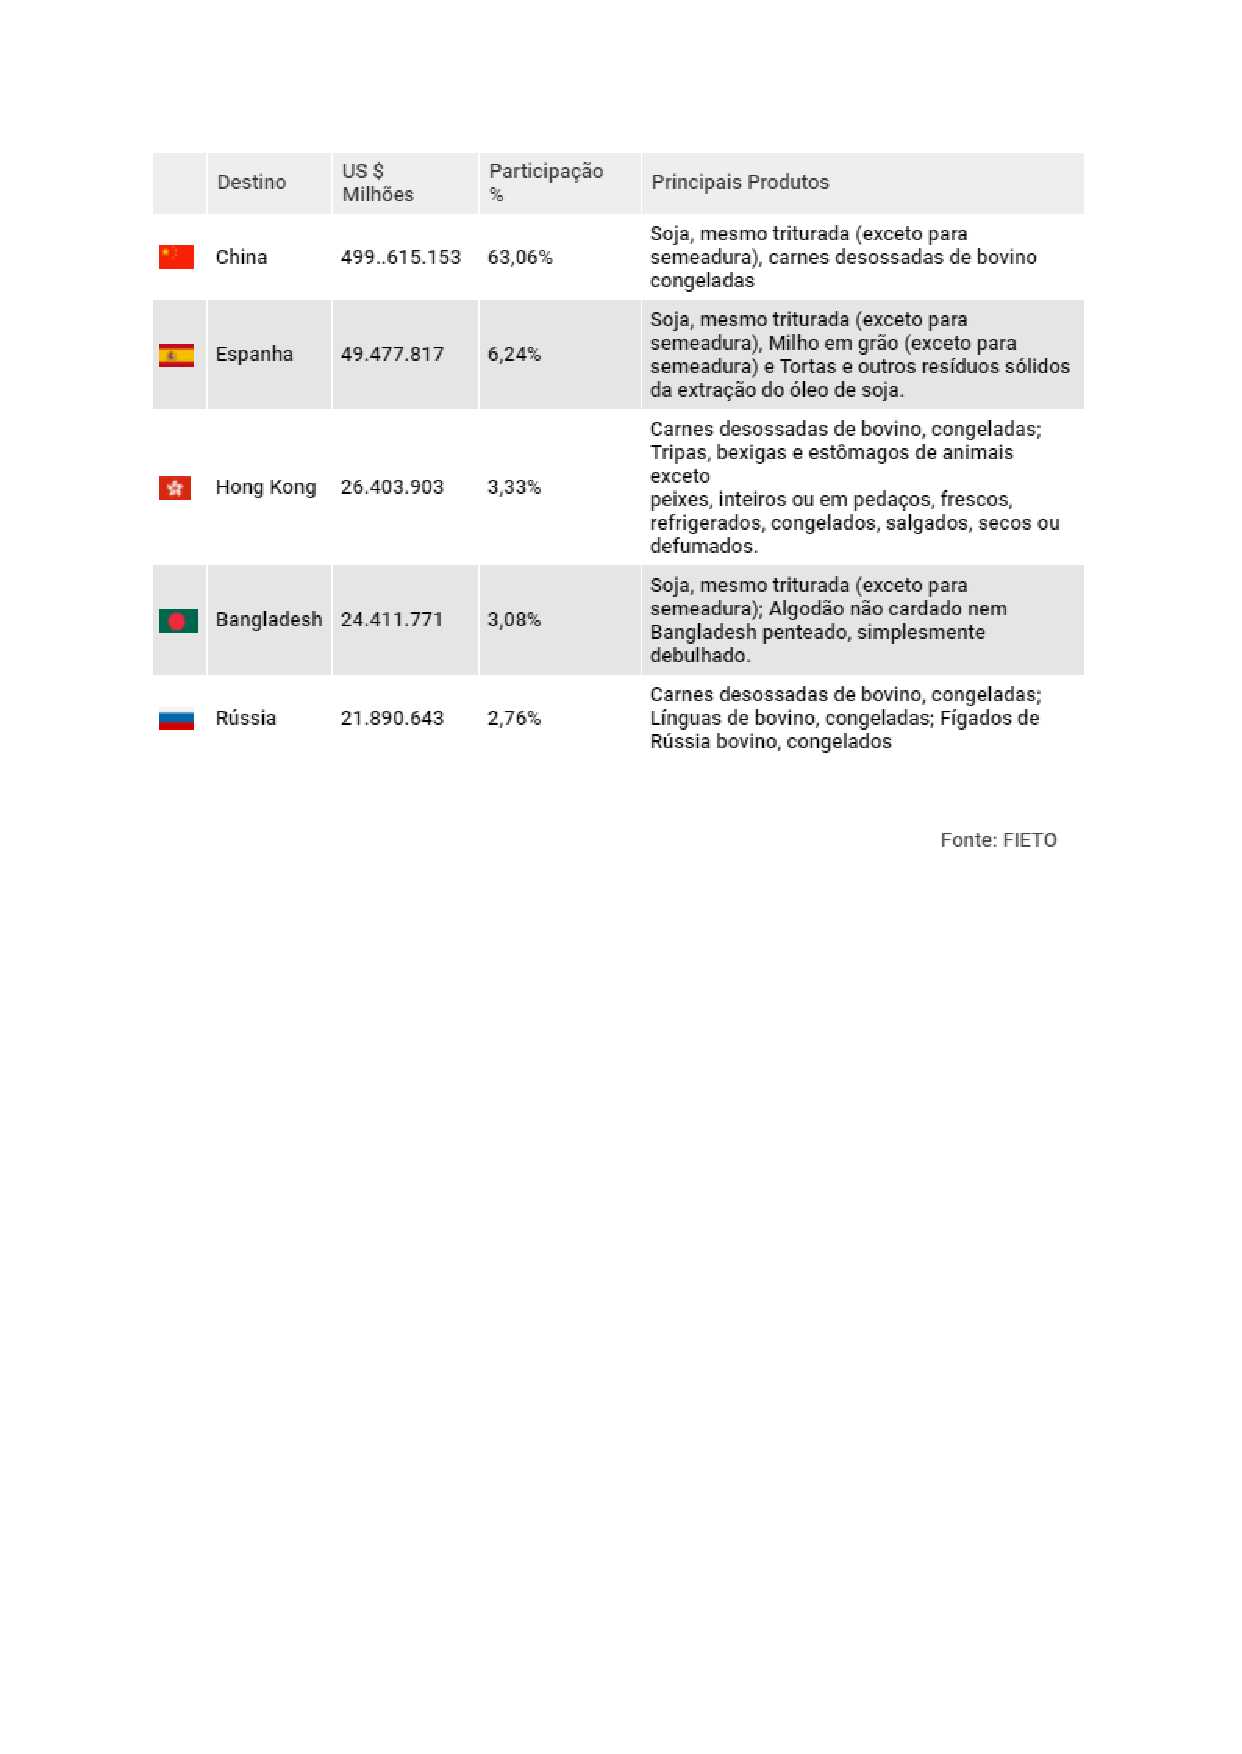
\includegraphics[width=.45\textwidth]{figs/tabela exportados.pdf}}}%
		\qquad
		\subfloat[\centering Origem]{{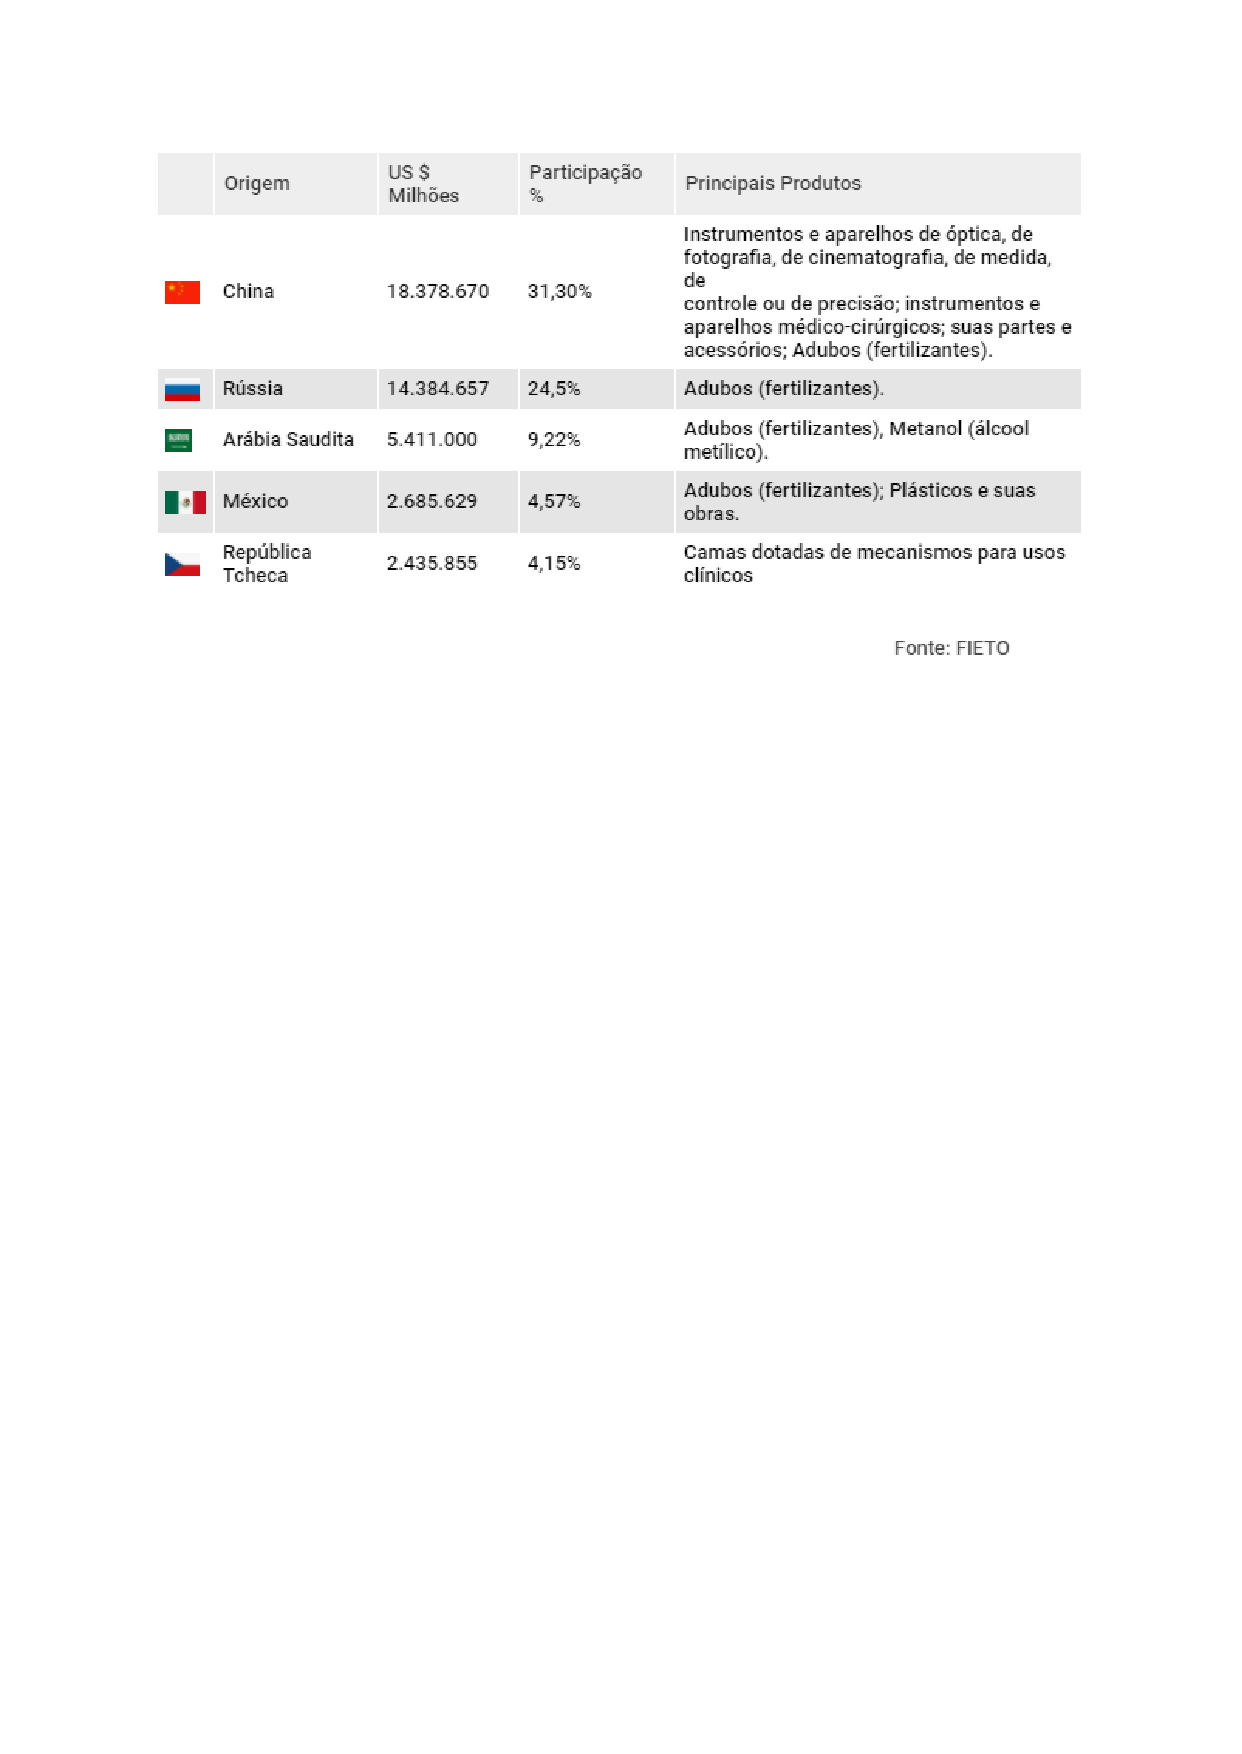
\includegraphics[width=.45\textwidth]{figs/tabela importados.pdf} }}%
	\end{figure}
\end{frame}

\begin{frame}
	\frametitle{Agronegócio}
	\begin{itemize}
		\item Importância da agricultura para a economia federal e estadual
		\item Produção
	\end{itemize}

\begin{figure}%
	\centering
	\subfloat[\centering Abate dos principais animais]{{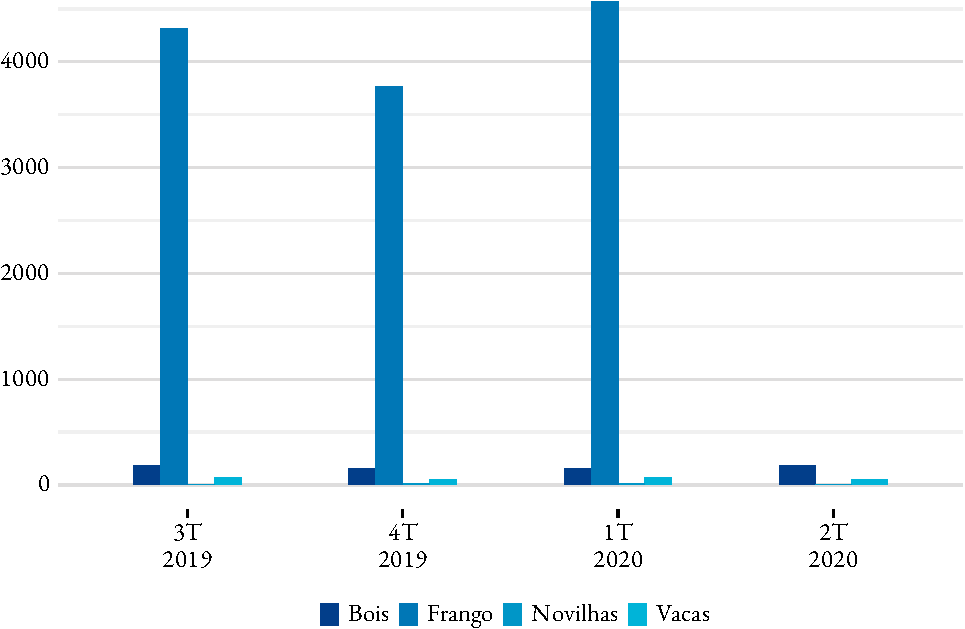
\includegraphics[width=.45\textwidth]{figs/abate.pdf}}}%
	\qquad
	\subfloat[\centering Produção nas lavouras]{{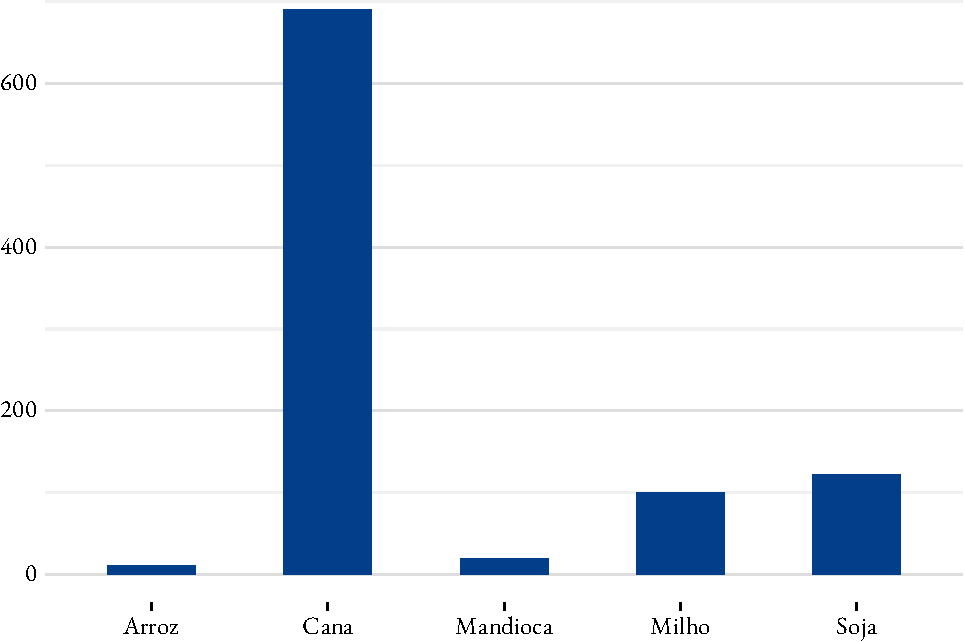
\includegraphics[width=.45\textwidth]{figs/produção.pdf} }}%
\end{figure}


\end{frame}


\begin{frame}
	\begin{center}
		\color{primarycolor}
		\textbf{OBRIGADO!}
	\end{center}
	
	
\end{frame}




\end{document}